\documentclass[12pt, notitlepage, final]{article} 

\newcommand{\name}{Vince Coghlan}

\usepackage{amsfonts}
\usepackage{amssymb}
\usepackage{amsmath}
\usepackage{latexsym}
\usepackage{enumerate}
\usepackage{amsthm}
\usepackage{nccmath}
\usepackage{setspace}
\usepackage[pdftex]{graphicx}
\usepackage{epstopdf}
\usepackage[siunitx]{circuitikz}
\usepackage{tikz}
\usepackage{float}
\usepackage{cancel} 
\usepackage{setspace}
\usepackage{overpic}
\usepackage{mathtools}
\usepackage{listings}
\usepackage{color}

\numberwithin{equation}{section}
\DeclareRobustCommand{\beginProtected}[1]{\begin{#1}}
\DeclareRobustCommand{\endProtected}[1]{\end{#1}}
\newcommand{\dbr}[1]{d_{\mbox{#1BR}}}
\newtheorem{lemma}{Lemma}
\newtheorem*{corollary}{Corollary}
\newtheorem{theorem}{Theorem}
\newtheorem{proposition}{Proposition}
\theoremstyle{definition}
\newtheorem{define}{Definition}
\newcommand{\column}[2]{
\left( \begin{array}{ccc}
#1 \\
#2
\end{array} \right)}

\newdimen\digitwidth
\settowidth\digitwidth{0}
\def~{\hspace{\digitwidth}}

\setlength{\parskip}{1pc}
\setlength{\parindent}{0pt}
\setlength{\topmargin}{-3pc}
\setlength{\textheight}{9.0in}
\setlength{\oddsidemargin}{0pc}
\setlength{\evensidemargin}{0pc}
\setlength{\textwidth}{6.5in}
\newcommand{\answer}[1]{\newpage\noindent\framebox{\vbox{{\bf ECEN 3400 Spring 2014} 
\hfill {\bf \name} \vspace{-1cm}
\begin{center}{Homework \#4}\end{center} } }\bigskip }

%absolute value code
\DeclarePairedDelimiter\abs{\lvert}{\rvert}%
\DeclarePairedDelimiter\norm{\lVert}{\rVert}
\makeatletter
\let\oldabs\abs
\def\abs{\@ifstar{\oldabs}{\oldabs*}}
%
\let\oldnorm\norm
\def\norm{\@ifstar{\oldnorm}{\oldnorm*}}
\makeatother

\def\dbar{{\mathchar'26\mkern-12mu d}}
\def \Frac{\displaystyle\frac}
\def \Sum{\displaystyle\sum}
\def \Int{\displaystyle\int}
\def \Prod{\displaystyle\prod}
\def \P[x]{\Frac{\partial}{\partial x}}
\def \D[x]{\Frac{d}{dx}}
\newcommand{\PD}[2]{\frac{\partial#1}{\partial#2}}
\newcommand{\PF}[1]{\frac{\partial}{\partial#1}}
\newcommand{\DD}[2]{\frac{d#1}{d#2}}
\newcommand{\DF}[1]{\frac{d}{d#1}}
\newcommand{\fix}[2]{\left(#1\right)_#2}
\newcommand{\ket}[1]{|#1\rangle}
\newcommand{\bra}[1]{\langle#1|}
\newcommand{\braket}[2]{\langle #1 | #2 \rangle}
\newcommand{\bopk}[3]{\langle #1 | #2 | #3 \rangle}
\newcommand{\Choose}[2]{\displaystyle {#1 \choose #2}}
\newcommand{\proj}[1]{\ket{#1}\bra{#1}}
\def\del{\vec{\nabla}}
\newcommand{\avg}[1]{\langle#1\rangle}
\newcommand{\piecewise}[4]{\left\{\beginProtected{array}{rl}#1&:#2\\#3&:#4\endProtected{array}\right.}
\newcommand{\systeme}[2]{\left\{\beginProtected{array}{rl}#1\\#2\endProtected{array}\right.}
\def \KE{K\!E}
\def\Godel{G$\ddot{\mbox{o}}$del}

\onehalfspacing

\begin{document}

\answer{}
1) \textbf{12.13:}
\begin{figure}[H]
\begin{center}
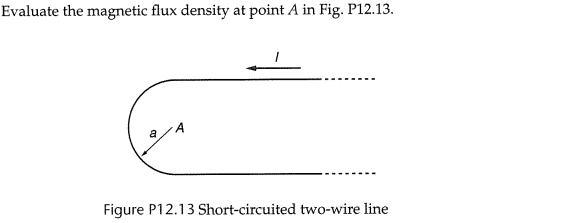
\includegraphics[width=14cm]{p1}
\end{center}
\end{figure}

We can find this by using an integral.  Since $l$ and $u_r$ are always normal to
eachother, the values of all the little $dB$s will compound together in the same
direction, and the cross products will be 1.  We are basically evaluating the
length of the wire from 0 to $\pi$.  Since the circumference of a circle is $2\pi a$
then $\frac{1}{2}$ of the circumference, and the value of the integral is just $\pi a$.
We get the following:
\[
  B_A = \int_{0}^{\pi} \frac{\mu_0}{4\pi}\frac{I}{a^2}dl = \frac{\mu_0I}{4a}
\]
\newpage
2) \textbf{12.38:}
\begin{figure}[H]
\begin{center}
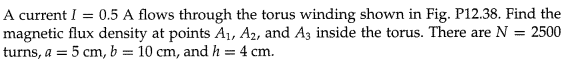
\includegraphics[width=14cm]{p2a}
\end{center}
\end{figure}
\begin{figure}[H]
\begin{center}
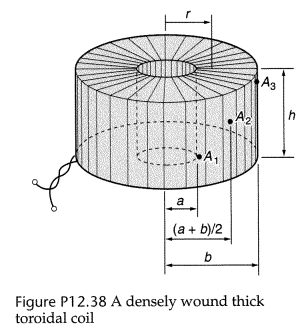
\includegraphics[width=8cm]{p2b}
\end{center}
\end{figure}

We can utilize ampere's law to find the magnetic field generally:
\[
  \oint_C B\cdot dl = \mu_0 \int_S J\cdot S \Rightarrow 2\pi rB = \mu_0 N I
\]
\[
  B_{A_1} = \frac{\mu_0 NI}{2\pi a}\text{, }B_{A_2} = \frac{\mu_0 NI}{\pi (a+b)}\text{, }B_{A_3} = \frac{\mu_0 NI}{2\pi b}
\]

\newpage
3) \textbf{13.5:}
\begin{figure}[H]
\begin{center}
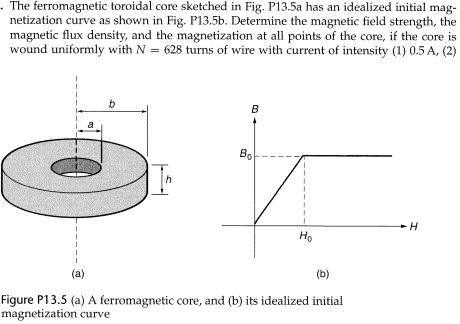
\includegraphics[width=14cm]{p3a}
\end{center}
\end{figure}
\begin{figure}[H]
\begin{center}
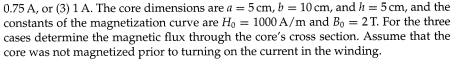
\includegraphics[width=14cm]{p3b}
\end{center}
\end{figure}

We will begin with Ampere's law (so we can find H).
\[
  \oint_C H\cdot dl = \int_S J\cdot dS
\]
I will first find the edges of where the magnetization curve applies.  If we are on the
left side of the magnetization curve, we can pull $H$ out of the integral and solve:
\[
  H 2\pi r = NI \Rightarrow H = \frac{N I}{2\pi r} \text{, } H<H_0
\]
Lets test to see if we are indeed on that side of the equation (using 0.5A):
\[
  H = \frac{NI}{2\pi a} = 999.5
\]
Since this will be the point of largest $H$, we know that for this case, we will never have to
deal with $M$.  I will finish out this case and then move on to the more complicated ones.  We know
the magnetic field strength to be:
\[
H = \frac{N I}{2\pi r}
\]
The Magnetic flus density $B$ is:
\[
B = \frac{\mu N I}{2\pi r}
\]
The magnetization is:
\[
  M = \frac{B}{\mu} - H = 0
\]
The flux $\Phi$ is:
\[
  \Phi = \int\int_S H \cdot dS = h\int_a^b  \frac{N I}{2\pi r} \cdot dr = \frac{hNI\ln(\frac{b}{a})}{2\pi} = 1.73 Wb
\]
Note that we can consider the field to be constant in the vertical direction, and so we only consider the
field as it changes around the radius $r$.  We will continue on to the next current, 1A:
\[
  H = \frac{NI}{2\pi b} = 999.5
\]
This is not that much smaller than 1000, so I will consider this to be the upper portion of the magnetization
curve.  This means that our value for $B$ is going to remain constant at 2T while our value for $H$
is going to increase with $M$.
\[
B = 2T
\]
\[
H = \frac{N I}{2\pi r}
\]
\[
  M = \frac{2T}{\mu} - H = \frac{2T}{\mu}-\frac{N I}{2\pi r}
\]
\[
  \Phi = \int\int_S H \cdot dS = h\int_a^b  \frac{N I}{2\pi r} \cdot dr = \frac{hNI\ln(\frac{b}{a})}{2\pi} = 3.46 Wb
\]
And for .75A we are going to have to use both equations for some point in between $r$ where:
\[
  H = \frac{NI}{2\pi r} = 1000
\]
We can solve and see that r = 0.0749 m.  This means that we must have two equations:
\begin{displaymath}
   B = \left\{
     \begin{array}{lr}
       \frac{\mu N I}{2\pi r} & : 0.05 < r < 0.0749\\
       2T & : 0.0749 < r < 0.10
     \end{array}
   \right.
\end{displaymath}
\begin{displaymath}
   M = \left\{
     \begin{array}{lr}
       0 & : 0.05 < r < 0.0749\\
       \frac{2T}{\mu}-\frac{N I}{2\pi r} & : 0.0749 < r < 0.10
     \end{array}
   \right.
\end{displaymath}
At this point the flux is going to be using the same equation, since $H$ is not dependent on these things,
and encompases only the field generated using Ampere's law, which is immune to this magnetisim tomfoolery.
\[
  \Phi = \int\int_S H \cdot dS = h\int_a^b  \frac{N I}{2\pi r} \cdot dr = \frac{hNI\ln(\frac{b}{a})}{2\pi} = 2.60 Wb
\]

4) \textbf{13.25:}
\begin{figure}[H]
\begin{center}
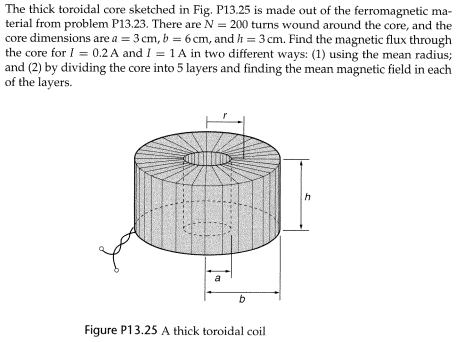
\includegraphics[width=14cm]{p4}
\end{center}
\end{figure}
\newpage
We will begin, as we often do, with Ampere's law:
\[
  \oint_C H\cdot dl = \int_S J\cdot dS
\]
\[
H = \frac{N I}{2\pi r}
\]
At I = 0.2 we can find the flux in two ways: The first way:
\[
  \Phi = H\cdot A = \frac{N I}{\pi (b-a)} h(b-a) = 0.38 Wb
\]
The other way is:
\[
  \frac{1}{6}\sum_{r=3.25,3.75,4.25,4.75,5.25,5.75} \frac{N I}{2\pi r} = 1.47 Wb
\]
At I = 1
\[
  \Phi = H\cdot A = \frac{N I}{\pi (b-a)} h(b-a) = 1.91 Wb
\]
\[
  \frac{1}{6}\sum_{r=3.25,3.75,4.25,4.75,5.25,5.75} \frac{N I}{2\pi r} = 7.35 Wb
\]

\newpage
5) \textbf{14.6:}
\begin{figure}[H]
\begin{center}
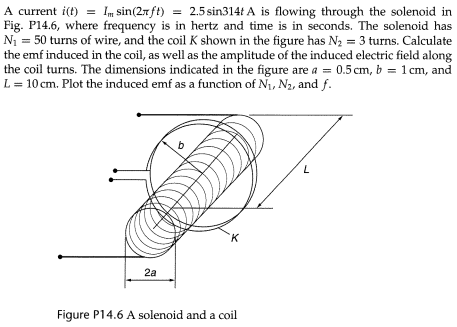
\includegraphics[width=14cm]{p5}
\end{center}
\end{figure}

We will use Faraday's law:
\[
  V = -\frac{d}{dt} \int_S B\cdot dS
\]
\[
  V = -\frac{d}{dt} \frac{\mu_0 N_1N_2i(t)2\pi a}{L}
\]
\[
  V = -\frac{d}{dt} \frac{\mu_0 N_1N_2I_m\sin(2\pi ft)2\pi a}{L}
\]
\[
  V = -\mu_0 N_1N_2I_m\cos(2\pi ft)4\pi^2af\frac{1}{L} \approx -9Vcos(314t)
\]
The induced emf will induce an electric field proportional to the resistance
of the wire, so the question cannot be answered numerically, but symbollically:
\[
  E_{max} = \frac{\mu_0 N_2 |V|}{2 R b}
\]
We know $|V|$ to be 9, but $R$ was not given in the problem. The plots will be the same
with respect to $N_1$ and $N_2$... so:
\begin{figure}[H]
\begin{center}
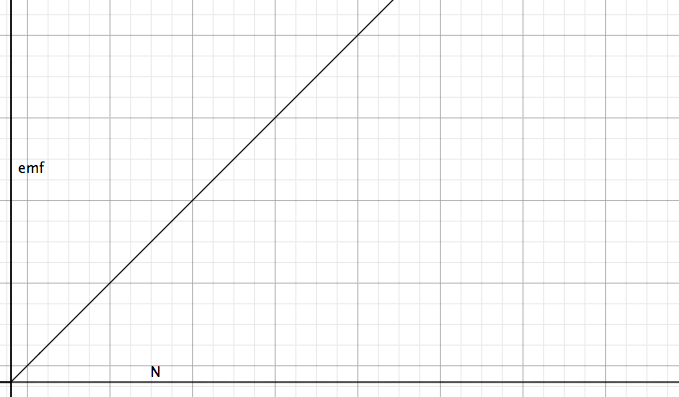
\includegraphics[width=14cm]{f1}
\end{center}
\end{figure}

And with frequency:
\begin{figure}[H]
\begin{center}
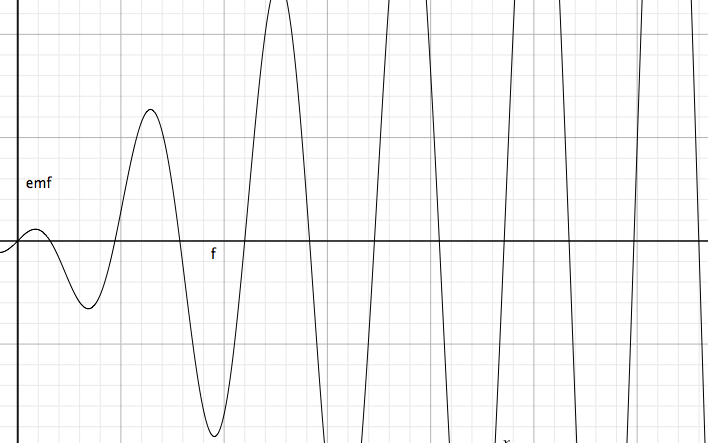
\includegraphics[width=14cm]{f2}
\end{center}
\end{figure}

\newpage
6) \textbf{14.16:}
\begin{figure}[H]
\begin{center}
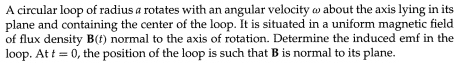
\includegraphics[width=14cm]{p6}
\end{center}
\end{figure}
First we find the flux to be:
\[
  \Phi = B(t)cos(\omega t)\pi a^2
\]
Then we can find the induced emf to be
\[
  V = -\frac{d}{dt}B(t)\cos(\omega t)\pi a^2
\]

7) \textbf{15.3:}
\begin{figure}[H]
\begin{center}
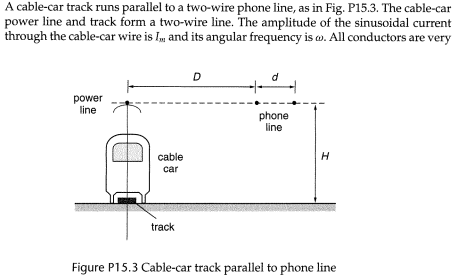
\includegraphics[width=14cm]{p7a}
\end{center}
\end{figure}
\begin{figure}[H]
\begin{center}
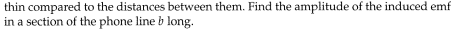
\includegraphics[width=14cm]{p7b}
\end{center}
\end{figure}
First we find the flux per unit length:
\[
  \Phi'_1 = \frac{\mu_0 i(t)}{2\pi} \int_{r_1}^{r_2} \frac{dr}{r} = \frac{\mu_0i(t)}{2\pi}\ln(\frac{r_2}{r_1})
\]
where $r_1 = D$ and $r_2 = \sqrt{D^2+H^2}$.  On the other line it is:
\[
  \Phi'_2 = \frac{\mu_0 i(t)}{2\pi} \int_{r_3}^{r_4} \frac{dr}{r} = \frac{\mu_0i(t)}{2\pi}\ln(\frac{r_4}{r_3})
\]
where $r_3 = D+d$ and $r_4 = \sqrt{(D+d)^2+H^2}$.  The total flux per unit length is thus:
\[
  \frac{\mu_0i(t)}{2\pi}\ln(\frac{r_2}{r_1}) + \frac{\mu_0i(t)}{2\pi}\ln(\frac{r_4}{r_3}) = \frac{\mu_0i(t)}{2\pi}\ln(\frac{r_2r_4}{r_1r_3})
\]
and our emf is:
\[
  -\frac{d}{dt}\frac{\mu_0i(t)}{2\pi}\ln(\frac{r_2r_4}{r_1r_3}) = -\frac{\omega\mu_0I_m\cos(\omega t)}{2\pi}\ln(\frac{r_2r_4}{r_1r_3})
\]

8) \textbf{15.10:}
\begin{figure}[H]
\begin{center}
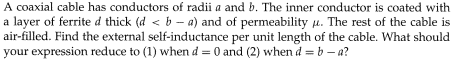
\includegraphics[width=14cm]{p8}
\end{center}
\end{figure}

We know from the textbook that the self inductance per unit length is:
\[
  L' = \frac{\mu_0}{2\pi}\ln(\frac{b}{a})
\]
With our new surface we will have to modify our equation to:
\[
  L' = \frac{\mu}{2\pi}\ln(\frac{a+d}{a}) + \frac{\mu_0}{2\pi}\ln(\frac{b}{a+d})
\]
It works much like a dielectric when capacitance is in question.

\end{document}
